\documentclass[aspectratio=169]{beamer}

\usetheme{Madrid}
\usecolortheme{default}

\usepackage[russian]{babel}
\usepackage{minted}
\usepackage{hyperref}
\usepackage{graphicx}

\title{Работа с запросами в JavaScript} 
\subtitle{и теория HTTP}
\author{Кормышев Егор ИСиП-301}
\date{\today}


\begin{document}

\frame{\titlepage}

% Frame 2: http requiests definitions 

\begin{frame}
  \frametitle{Определение HTTP запроса}
  
  \bigskip
  
  \large\textcolor{blue}{HTTP-запрос} - \normalsize Обмен данными между клиентом и сервером
  
  \bigskip

  \begin{center}
    \large Виды HTTP-сообщений
  \end{center}

  \begin{columns}
    % Request
    
    \begin{column}{0.5\textwidth}
      \centering
      \large \textbf{Запрос (Request)}
      % Client -> Server image
      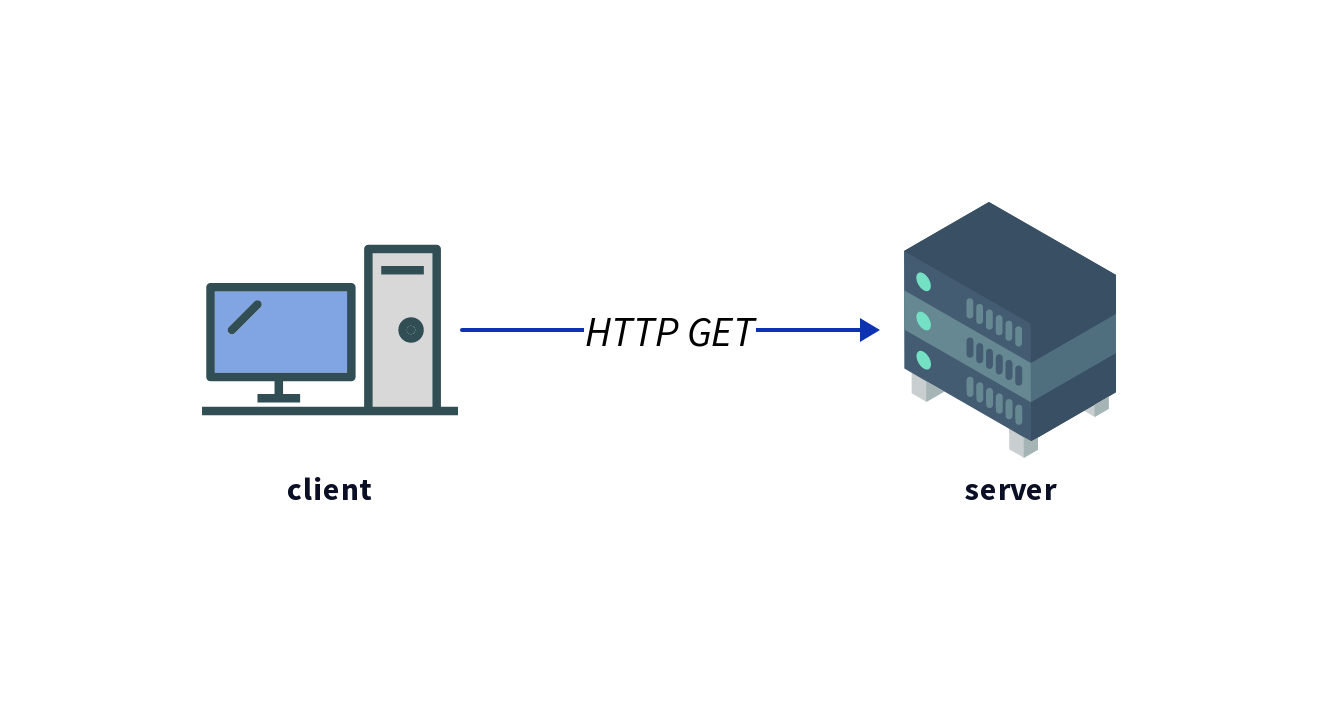
\includegraphics[width=1.2\textwidth]{assets/request.png}
    \end{column}
    
    % Response
    
    \begin{column}{0.5\textwidth}
      \centering
      \large \textbf{Ответ (Response)}
      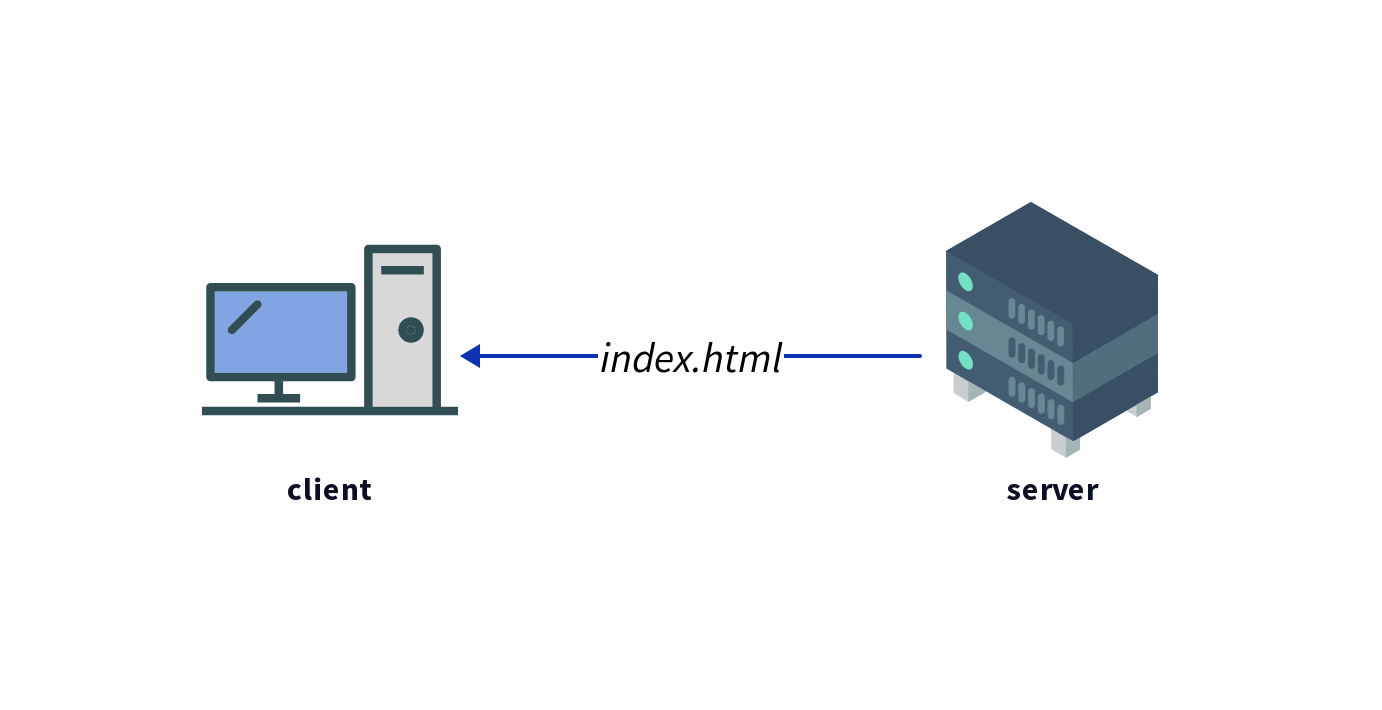
\includegraphics[width=1.2\textwidth]{assets/response.png}
    \end{column}

  \end{columns}


\end{frame}

% Frame 3: HTTP Request parts

\begin{frame}
  \frametitle{Структура HTTP запроса}
  \begin{center}
    HTTP-запрос состоит из нескольких частей:
    \bigskip
    \begin{itemize}
    \item Строка запроса - \texttt{https://example.com}
    \item Заголовки (headers) - \texttt{\{ \\
        Accept: application/json \\
        User-Agent: Mozilla/5.0 \\
        Host: example.com \\
        ... \\
        \}}
      
    \item Тело запроса (body) - данные, передаваемые серверу при запросе в формате json/xml/text
      
    \end{itemize}
  \end{center}
\end{frame}

% Frame 4: HTTP response

\begin{frame}
  \frametitle{Структура HTTP ответа}

  \begin{center}
    HTTP-ответ состоит из нескольких частей:
    \bigskip
    \begin{itemize}
    \item Строка ответа - \texttt{HTTP/1.1 200 OK}
    \item Заголовки (headers) - \texttt{\{ \\
        Accept: application/json \\
        User-Agent: Mozilla/5.0 \\
        Host: example.com \\
        ... \\
        \}}
      
    \item Тело запроса (body) - данные, передаваемые от сервера в формате json/html/text
      
    \end{itemize}
  \end{center}
  
\end{frame}

% Frame 5: HTTP Response codes

\begin{frame}
  \frametitle{Коды статуса HTTP-ответа}
  \begin{center}
    Все коды делятся на 5 групп:
  \end{center}
  
  \begin{itemize}
  \item 1.x.x - Информация
  \item 2.x.x - Успех
  \item 3.x.x - Перенаправление
  \item 4.x.x - Клиентская ошибка
  \item 5.x.x - Серверная ошибка
  \end{itemize}
  
  \begin{center}
    Подробнее в \textcolor{blue}{\underline{\href{assets/codes.png}{таблице}}}
  \end{center}
  
\end{frame}

% Frame 6: GET request in js/ts

\begin{frame}
  \frametitle{Программируемые запросы в js/ts}
  \begin{center}
    Способы выполнения HTTP запроса в javascript:
  \end{center}
  \begin{itemize}
  \item Стандартная фунцкия \texttt{fetch()}
  \item Библиотека \texttt{axios}
  \end{itemize}

  
\end{frame}

% Frame 7: JS/TS fetch example

\begin{frame}[fragile]
  \frametitle{Использование функции \texttt{fetch()}}
  \begin{center}
    \begin{block}{Пример запроса в \texttt{js}}
      \begin{minted}{javascript}
        fetch(url)
        .then(promise => {
          return promise.json()
          .then(data => {
            console.log(data)
          }).catch(err => {
            console.log(err)
          })
        })
        .catch(err => {
          console.log(err)
        })

      \end{minted}
    \end{block}
  \end{center}
\end{frame}

% Frame 8: fetch structure

\begin{frame}[fragile]
  \frametitle{Структура функции fetch}
  \begin{center}
    Структура функции fetch:
  \end{center}
  \begin{enumerate}
  \item \texttt{fetch(url)} - запрос
  \item \texttt{then(res)} - \underline{результат} запроса
  \item \texttt{catch(err)} - объект ошибки
  \end{enumerate}
\end{frame}

% Frame 9: Types in fetch 

\begin{frame}[fragile,allowframebreaks]
  \frametitle{fetch in typescript}
  \begin{block}{Типы в fetch}
    \begin{minted}{typescript}

      export interface Root {
        id: number
        name: string
        username: string
        email: string
        address: Address
        phone: string
        website: string
        company: Company
      }
      {...}
    \end{minted}
  \end{block}

  \begin{block}{Типы в fetch II}
    \begin{minted}{typescript}

      let url = "https://jsonplaceholder.typicode.com/users";

      fetch(url)
      .then((promise: Response) => {
        return promise.json() as Promise<User[]>;
      })
      .then((data: User[]) => {
        console.log(data);
      })
      .catch((err: Error) => {
        console.log(err);
      });

    \end{minted}
    \end{block}
  
\end{frame}

\end{document}
